\section{Results}\label{sec:results}
\subsection{Real ToF noise characterisation (SQ1)}\label{sec:res-noise}
The planar protocol shows that axial precision is sub-millimetre and essentially flat with
range, with no Kinect-style growth (Table~\ref{tab:axial}, Figure~\ref{fig:sigma}).
Fitting the expected quadratic $\sigma_z(z)=a+bz^2$ gives $a=0.91$\,mm and a slightly
\emph{negative} curvature ($b\approx-0.49\,\mathrm{mm\,m^{-2}}$), so the Nguyen range model
\cite{nguyen2012modeling} does not apply here; the OAK-D's multi-frequency phase unwrapping
yields unusually quiet bulk depth (about $0.6$--$0.7$\,mm, against the $2$--$10$\,mm typical
of Kinect-class sensors). Bias stays within $\pm3$\,mm.

\begin{table}[t]
\centering
\caption{Planar axial precision versus distance (200 frames, $n\approx33{,}920$ px per
distance).}
\label{tab:axial}
\footnotesize
\begin{tabular}{lccccc}
\toprule
Distance (m)   & 0.40 & 0.50 & 0.60 & 0.70 & 0.80 \\
Axial $\sigma$ (mm) & 0.87 & 0.80 & 0.68 & 0.55 & 0.69 \\
\bottomrule
\end{tabular}
\end{table}

\begin{figure}[t]
\centering
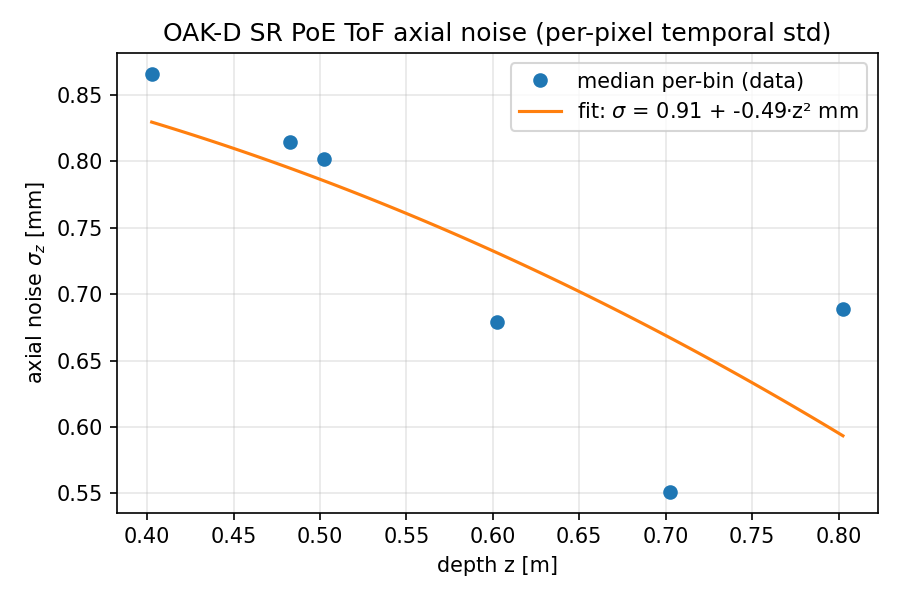
\includegraphics[width=\linewidth]{sigma_vs_z.png}
\caption{Axial depth precision $\sigma_z$ versus distance ($0.40$--$0.80$\,m). The profile
is sub-millimetre and flat (a slightly negative fitted curvature), so the range-growing
Nguyen model does not describe this multi-frequency ToF sensor.}
\label{fig:sigma}
\end{figure}

The object protocol locates the real, pose-relevant noise at object edges rather than on
their bodies (Table~\ref{tab:edge}, Figure~\ref{fig:overlays}). Body noise stays quiet on
all objects, but the six-pixel edge ring is dominated by flying pixels, with rates from
53\% to 99\%. This motivates both the median-centroid estimator and the inclusion of an
edge mixed-pixel term in the injector. Three caveats apply: the simple ``sharp edges are
clean, curved edges are noisy'' story is too strong, since the sharp box still shows
94.9\%; the can is low mainly because it is the largest object; and the rate is computed
over a fixed six-pixel ring, so it is partly size-sensitive and is reported qualitatively.

\begin{table}[t]
\centering
\caption{Per-object body noise and edge flying-pixel rate.}
\label{tab:edge}
\footnotesize
\begin{tabular}{lccc}
\toprule
Object & Body $\sigma$ (mm) & Dropout & Edge flying-pixel \\
\midrule
coke\_can  & 0.70 & 0\% & 53.1\% \\
banana     & 0.62 & 0\% & 98.7\% \\
golf\_ball & 0.65 & 0\% & 98.2\% \\
blue\_box  & 0.71 & 0\% & 94.9\% \\
\bottomrule
\end{tabular}
\end{table}

\begin{figure}[t]
\centering
\begin{subfigure}{0.49\linewidth}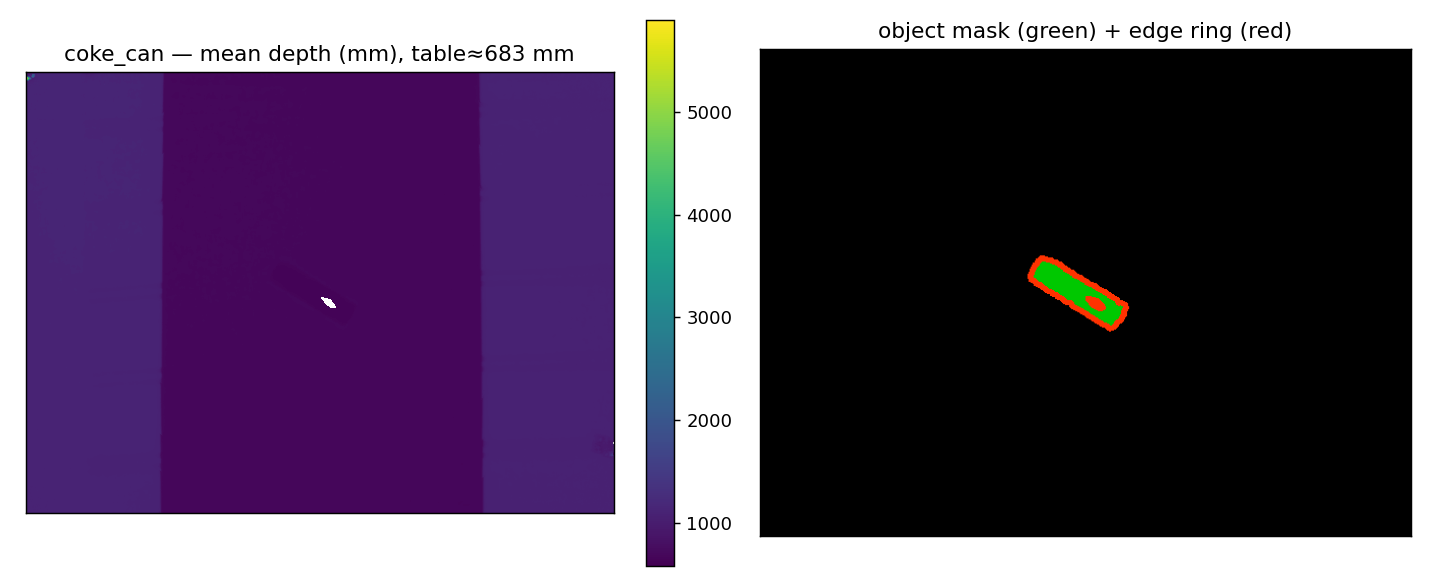
\includegraphics[width=\linewidth]{coke_can_overlay.png}\caption{coke\_can (53.1\%)}\end{subfigure}\hfill
\begin{subfigure}{0.49\linewidth}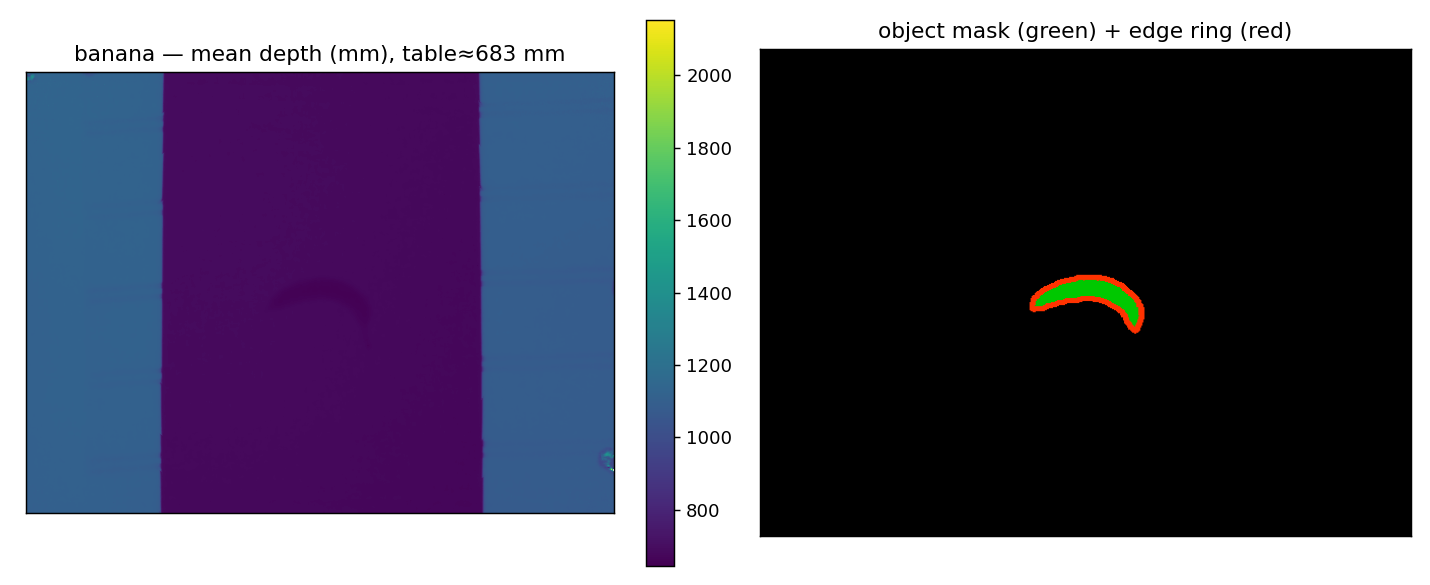
\includegraphics[width=\linewidth]{banana_overlay.png}\caption{banana (98.7\%)}\end{subfigure}
\\[2pt]
\begin{subfigure}{0.49\linewidth}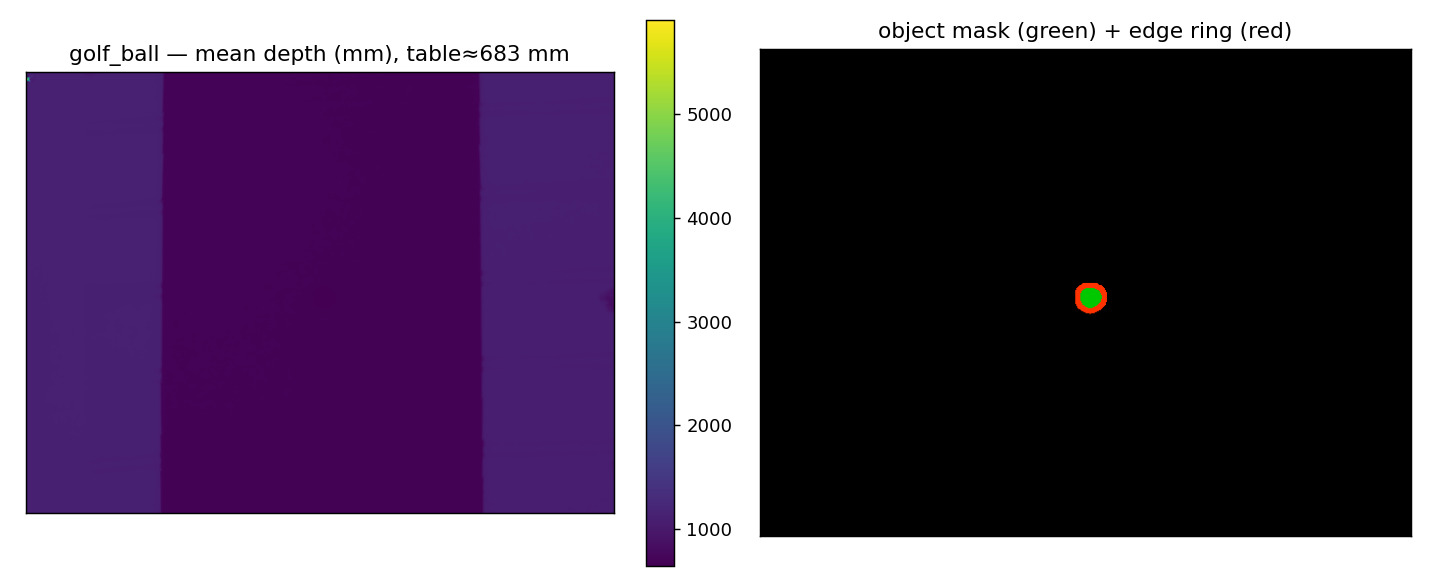
\includegraphics[width=\linewidth]{golf_ball_overlay.png}\caption{golf\_ball (98.2\%)}\end{subfigure}\hfill
\begin{subfigure}{0.49\linewidth}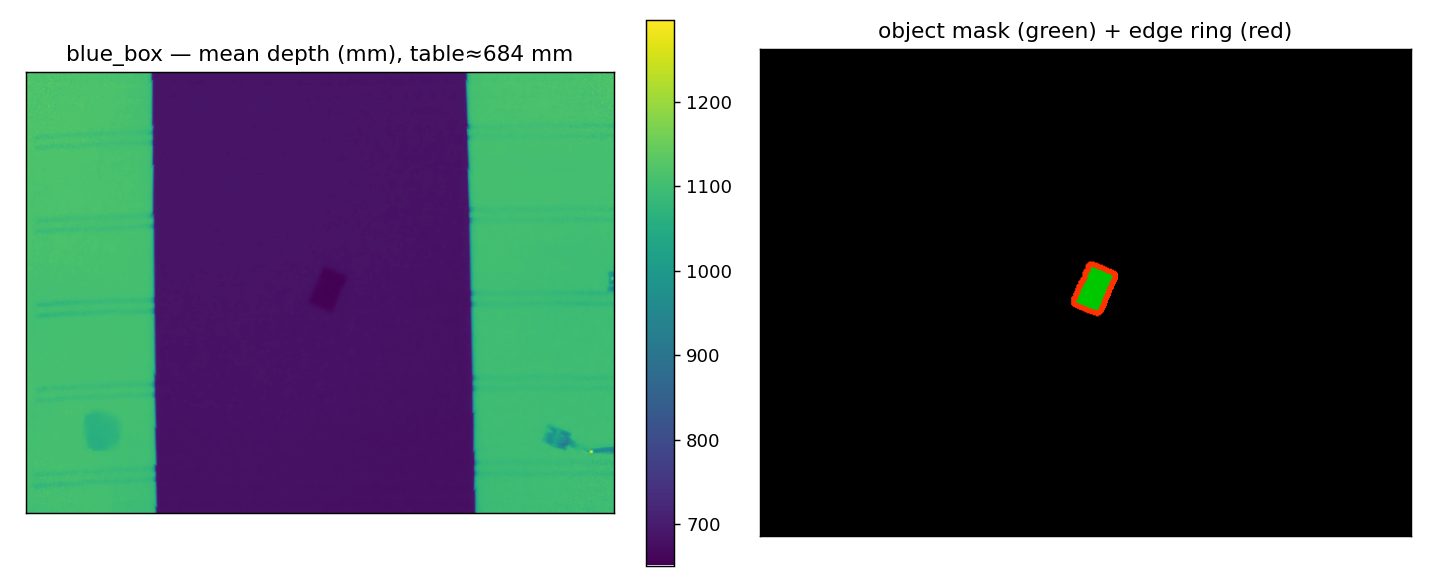
\includegraphics[width=\linewidth]{blue_box_overlay.png}\caption{blue\_box (94.9\%)}\end{subfigure}
\caption{Per-object edge overlays: the quiet body (green) versus the thin edge ring of
flying/mixed pixels (red). The pose-relevant noise lives almost entirely at the edges,
which the median centroid discards.}
\label{fig:overlays}
\end{figure}

\subsection{Noise injection and pose accuracy (SQ2)}\label{sec:res-inject}
At the measured noise level, injected noise has no measurable effect on pose accuracy. The
measured condition ($\times1$) is indistinguishable from clean and from the literature
model, and the planar (table-XY) RMSE stays flat at roughly $3.5$\,mm through $\times10$
(Table~\ref{tab:pose}, Figure~\ref{fig:posevsnoise}). The only visible movement below
$\times10$ is a small creep in the 3D RMSE, which is the axial (Z) component; the planar
difference between clean and $\times1$ is below $0.1$\,mm.

\subsection{Axial-scale ablation}\label{sec:res-ablation}
The same data are the ablation. Accuracy only degrades once the axial term is scaled to
about ten times the measured level (an axial $\sigma$ of roughly $9$\,mm), and all four
objects collapse together at $\times20$. This is the key verification that the null is real
rather than a broken pipeline: the injector does eventually break perception, but only an
order of magnitude above reality. That level is not merely hypothetical: an axial
$\sigma$ near $9$\,mm is representative of ToF operation in adverse conditions---strong
ambient infrared (e.g.\ direct sunlight), hot or industrial settings, airborne
particulates, and specular or low-reflectivity surfaces
\cite{foix2011lockin,sarbolandi2015kinect}---so the ablation also locates the regime in
which depth-noise fidelity would begin to matter (discussed in
Section~\ref{sec:disc-scope}).

\begin{table}[t]
\centering
\caption{Pose RMSE (mm) as planar\,/\,3D, by object and axial scale ($\times1$ is the
measured level). Values are flat from clean through $\times10$ and collapse at $\times20$.}
\label{tab:pose}
\footnotesize
\setlength{\tabcolsep}{4pt}
\resizebox{\columnwidth}{!}{%
\begin{tabular}{lcccc}
\toprule
Axial scale & coke\_can & banana & golf\_ball & blue\_box \\
\midrule
0 (clean)       & 3.31\,/\,4.85 & 8.71\,/\,10.67 & 4.77\,/\,7.89  & 3.06\,/\,3.06 \\
$\times1$       & 3.45\,/\,4.99 & 8.60\,/\,10.64 & 4.66\,/\,7.94  & 3.44\,/\,3.44 \\
$\times5$       & 3.53\,/\,6.03 & 8.68\,/\,11.12 & 4.53\,/\,8.55  & 3.63\,/\,3.71 \\
$\times10$      & 3.47\,/\,7.41 & 9.08\,/\,12.19 & 4.39\,/\,10.48 & 3.44\,/\,4.03 \\
$\times20$      & 9.55\,/\,18.43 & 22.43\,/\,24.53 & 8.58\,/\,19.08 & 8.68\,/\,10.21 \\
\bottomrule
\end{tabular}}
\end{table}

\begin{figure}[t]
\centering
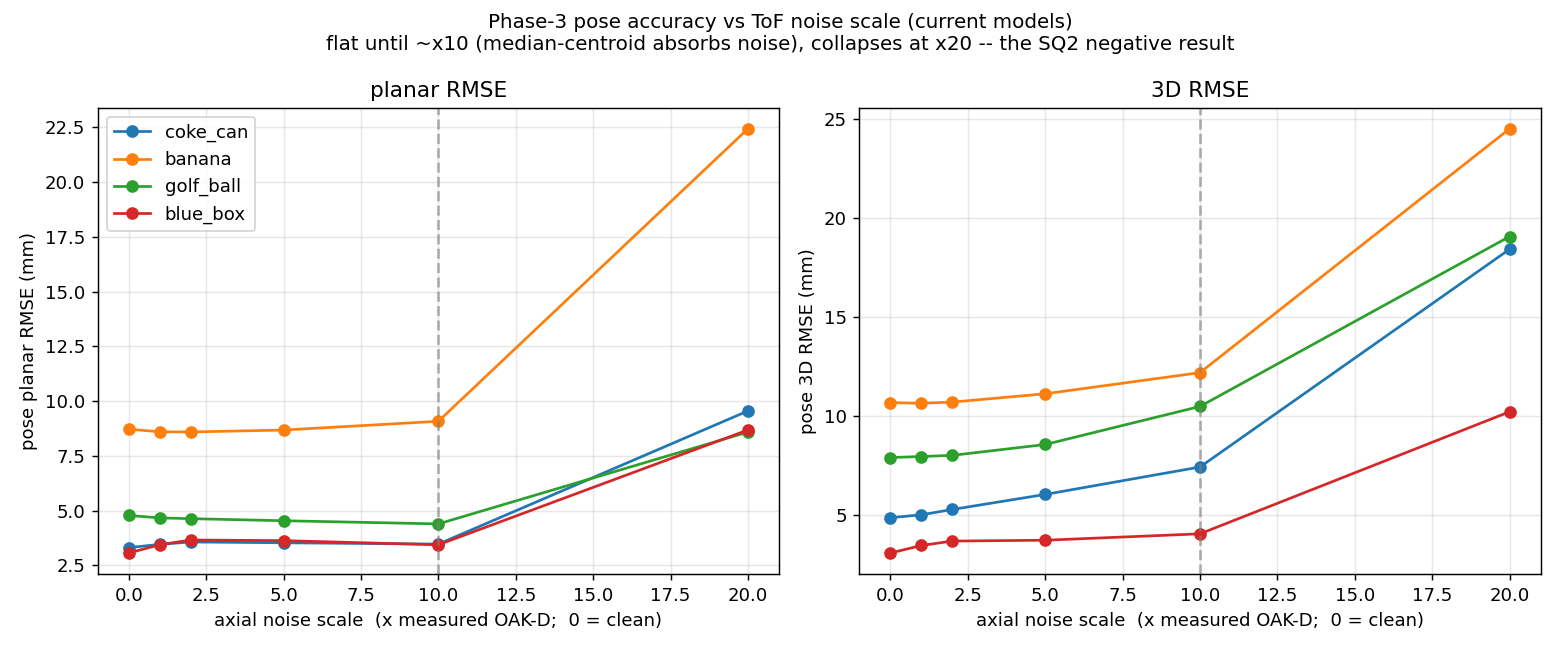
\includegraphics[width=\linewidth]{phase3_pose_vs_noise.png}
\caption{Pose RMSE versus axial noise scale for the four objects: flat from clean through
$\times10$, then a sharp collapse at $\times20$. Realistic noise ($\times1$) sits an order
of magnitude below the threshold at which the estimator degrades.}
\label{fig:posevsnoise}
\end{figure}

\subsection{Simulated manipulation (SQ3, simulation)}\label{sec:res-simmanip}
The simulated grasp results echo the pose threshold (Table~\ref{tab:grasp},
Figure~\ref{fig:rate}). All four objects are detected in every trial, so accuracy rather
than detection is the bottleneck. The three graspable objects are flat from clean through
$\times10$ and collapse only at $\times20$. Per-object behaviour is governed by the clean
error against the jaw tolerance: the blue box (${\sim}3.5$\,mm error against a $7.5$\,mm
tolerance) is at 100\%; the golf ball (${\sim}5.2$ against $6.0$) and banana
(${\sim}9.3$ against $10$) sit on their tolerance boundaries at 65\%; and the can
(${\sim}4.9$ against $1.5$) is floored at 0\%, a size limit ($52$\,mm body in a $55$\,mm
jaw) rather than a noise effect.

\begin{table}[t]
\centering
\caption{Analytic \texttt{grasp\_feasible} success rate (\%), $N=20$ per cell. Jaw
tolerance per object in parentheses.}
\label{tab:grasp}
\footnotesize
\setlength{\tabcolsep}{4pt}
\resizebox{\columnwidth}{!}{%
\begin{tabular}{lccccc}
\toprule
Condition & coke & banana & golf & blue\_box & Overall \\
          & (1.5) & (10) & (6) & (7.5) & \\
\midrule
clean         & 0  & 65 & 65 & 100 & 57.50 \\
$\times1$     & 5  & 65 & 65 & 100 & 58.75 \\
$\times10$    & 0  & 65 & 75 & 100 & 60.00 \\
$\times20$    & 5  & 30 & 20 & 50  & 26.25 \\
\bottomrule
\end{tabular}}
\end{table}

\begin{figure}[t]
\centering
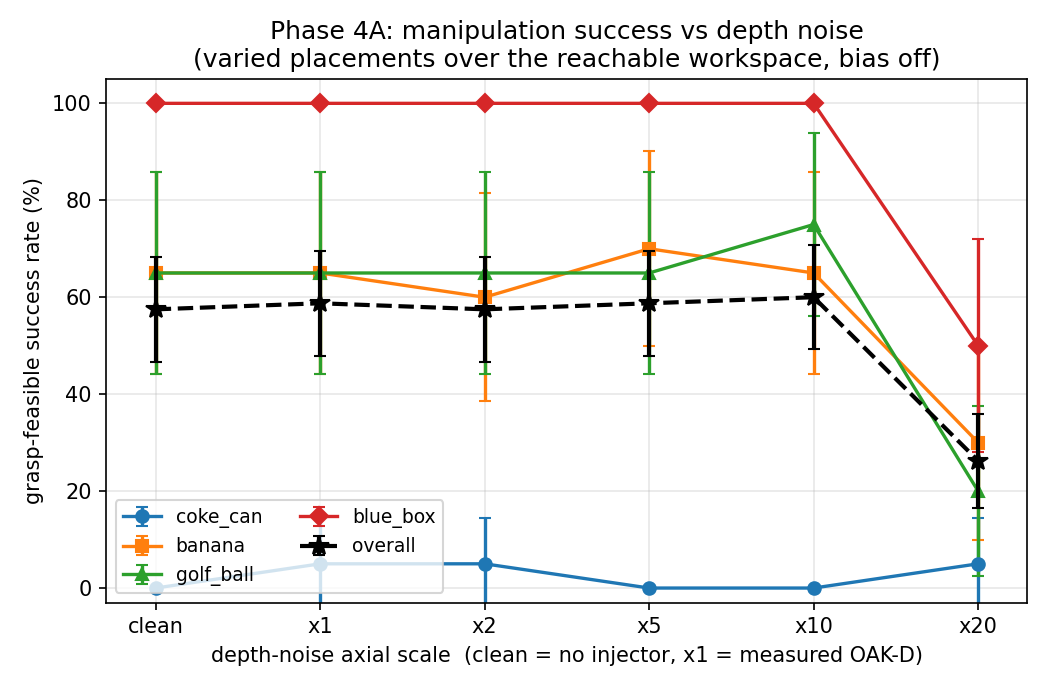
\includegraphics[width=\linewidth]{phase4a_rate_vs_axial_scale.png}
\caption{Analytic grasp-feasible success versus axial noise scale, per object. The three
graspable objects are flat clean$\rightarrow\times10$ and collapse at $\times20$; the can
is floored by a size limit independent of noise.}
\label{fig:rate}
\end{figure}

\subsection{Real pose gap and real manipulation (SQ3, real)}\label{sec:res-real}
The negative result carries onto the real system. The measured real-versus-sim planar pose
gap is small for every object, between $-1.4$ and $+3.6$\,mm (Table~\ref{tab:gap},
Figure~\ref{fig:gap}), and \texttt{sim\_clean} remains indistinguishable from
\texttt{sim\_noisy\_oakd} on real data. The simulated reference here is the
varied-placement sweep of Section~\ref{sec:res-simmanip}, whose wider pose spread raises
planar RMSE relative to the central scenes of Table~\ref{tab:pose}; this is why the
\texttt{sim\_clean} values differ between the two tables. The one positive outlier is the
blue box ($+3.6$\,mm), which becomes relevant for grasping.

\begin{table}[t]
\centering
\caption{Real-versus-sim planar pose RMSE (mm). The gap is computed as
real\,$-$\,\texttt{sim\_clean}.}
\label{tab:gap}
\footnotesize
\setlength{\tabcolsep}{4pt}
\resizebox{\columnwidth}{!}{%
\begin{tabular}{lcccc}
\toprule
Condition & coke\_can & banana & golf\_ball & blue\_box \\
\midrule
sim\_clean ($n{=}20$)      & 10.44 & 13.27 & 6.15 & 3.78 \\
sim\_noisy\_oakd ($n{=}20$) & 10.35 & 13.24 & 6.02 & 3.54 \\
real ($n{=}4$)             & 9.38 & 12.13 & 4.75 & 7.42 \\
\midrule
Gap (real $-$ sim\_clean)  & $-1.1$ & $-1.1$ & $-1.4$ & $+3.6$ \\
\bottomrule
\end{tabular}}
\end{table}

\begin{figure}[t]
\centering
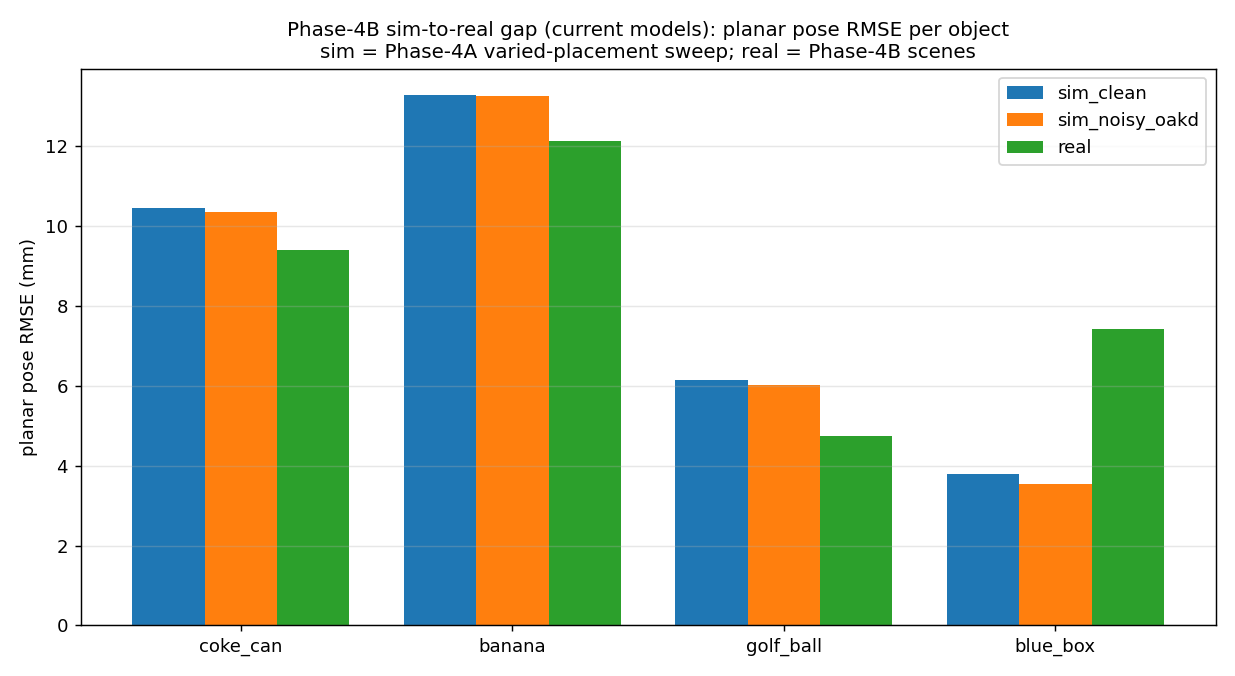
\includegraphics[width=\linewidth]{phase4b_sim_to_real_gap.png}
\caption{Real versus simulated planar pose RMSE per object (clean sim, noisy sim, real).
The real bars land close to the simulated ones, and clean and noisy simulation remain
indistinguishable: the negative result carries end-to-end on real data.}
\label{fig:gap}
\end{figure}

For real manipulation, all four objects were run under closed-loop control at five
near-zone placements with three repeats each, for 60 trials (Table~\ref{tab:phase4c},
Figure~\ref{fig:realpred}). The blue box reached 11/15 (73\%), the banana and coke can both
10/15 (67\%), and the golf ball 3/15 (20\%), for an overall $34/60=57\%$ lift-and-hold. The
most informative feature is that these rates follow neither the Phase-4A analytic
feasibility ceiling nor the Phase-4B pose-error-versus-tolerance predictor; they diverge
from both, and in both directions. Once the visual loop has driven the in-frame aiming
error to the camera floor (about $1$--$3$\,mm for every object in the near zone), the
residual variance is set by grip mechanics---object shape against the parallel-jaw closing
force and compliance---rather than by perception or aim.

The coke can is the clearest case. Its analytic feasibility is 0\% and its $1.5$\,mm rigid
centring tolerance predicts ``${\sim}0\%$'', yet it grasped 67\% of the time, so the real
arm out-performs the simulator: the loop centres the gripper to about $1$\,mm, and the firm
commanded close (well past the $52$\,mm body) stalls against the slightly compliant can with
enough force to secure it, an effect the rigid feasibility metric cannot represent. The
golf ball is the opposite. Its predictor was the most favourable of the four
($4.8<6.0$\,mm, ``likely''), yet it reached only 20\%, because a smooth sphere makes point
contact and rolls out of flat parallel jaws even when the aim converges below $2$\,mm; the
closed loop fixes the aim that was golf's wall but cannot supply a form-closure that flat
jaws do not afford a sphere. The banana (67\%) likewise exceeds its planar-RMSE prediction,
the elongated body being forgiving along its length. The blue box (73\%) is the only object
the predictor ``called''; within the validated near-zone ($r\le0.20$\,m, placements p1, p3,
p5) it grasped $9/9=100\%$, and every failure occurred at the far edge ($r\ge0.22$\,m), where
the high-mounted gripper marker loses tracking gain (Table~\ref{tab:bluebox}).

\begin{table*}[t]
\centering
\caption{Phase-4C real lift-and-hold success on the physical arm (60 trials), beside the
Phase-4A analytic feasibility ceiling and the Phase-4B pose-error-versus-tolerance
predictor. Intervals are Wilson 95\% score intervals.}
\label{tab:phase4c}
\footnotesize
\begin{tabular}{lccccccc}
\toprule
Object & $N$ & lift $k$ & rate (\%) & 95\% CI & sim-feas.\ (\%) & pose err (mm) & jaw tol (mm) \\
\midrule
blue\_box  & 15 & 11 & \textbf{73} & $[48,89]$ & 100 & 7.4  & 7.5 \\
banana     & 15 & 10 & \textbf{67} & $[42,85]$ & 65  & 12.1 & 10.0 \\
coke\_can  & 15 & 10 & \textbf{67} & $[42,85]$ & 0   & 9.4  & 1.5 \\
golf\_ball & 15 & 3  & \textbf{20} & $[7,45]$  & 65  & 4.8  & 6.0 \\
\midrule
\textbf{overall} & 60 & 34 & \textbf{57} & $[44,68]$ & --- & --- & --- \\
\bottomrule
\end{tabular}
\end{table*}

\begin{figure*}[t]
\centering
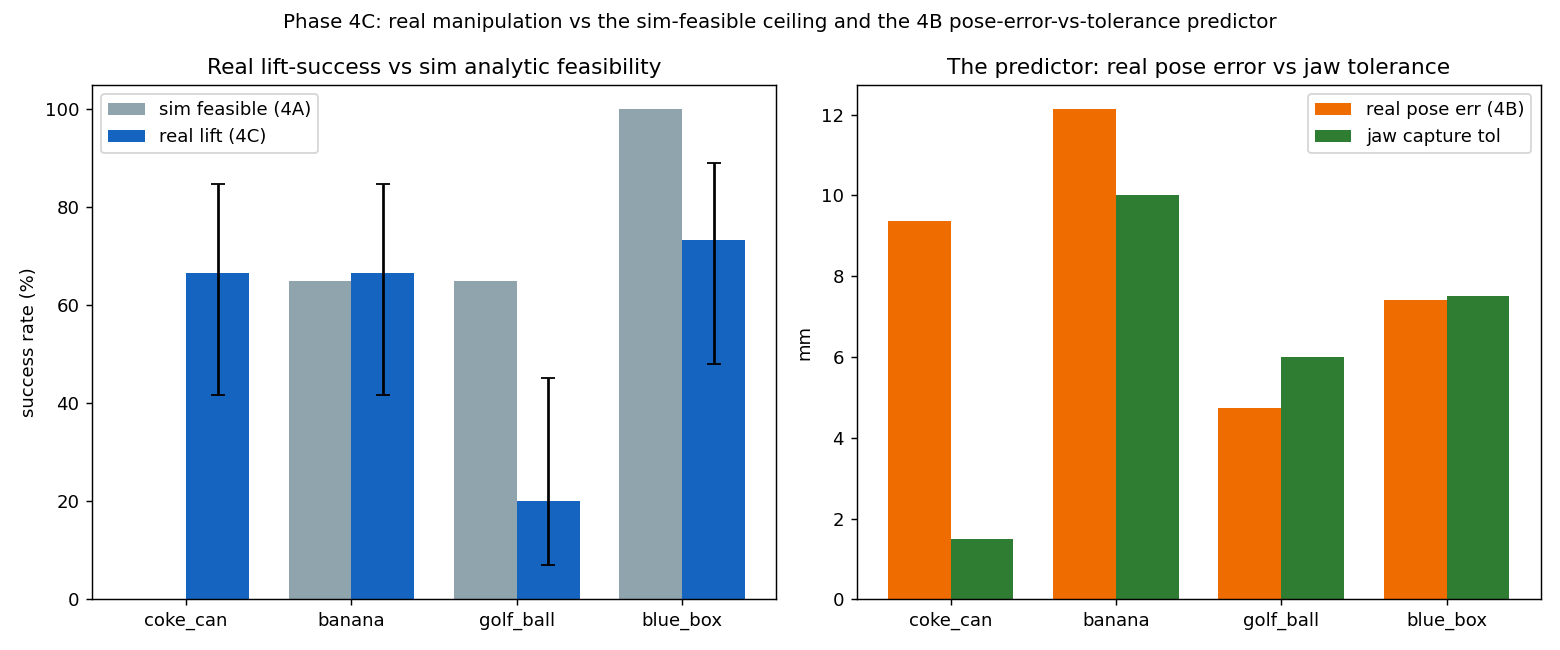
\includegraphics[width=0.9\textwidth]{phase4c_real_vs_pred.png}
\caption{Phase-4C real manipulation. \emph{Left:} real lift-success (with Wilson 95\%
intervals) against the Phase-4A analytic feasibility ceiling; the coke can has no
feasibility bar (0\%) yet grasps 67\%, while the golf ball has a 65\% ceiling yet only 20\%
real success. \emph{Right:} the Phase-4B planar pose error against each object's jaw
tolerance, which likewise fails to order the real rates---success is set by grip mechanics,
not aim.}
\label{fig:realpred}
\end{figure*}

\begin{table}[t]
\centering
\caption{Phase-4C closed-loop blue-box trials (5 placements $\times$ 3 repeats). The servo
column is the table-frame alignment error before$\rightarrow$after the visual nudge (mm).}
\label{tab:bluebox}
\footnotesize
\setlength{\tabcolsep}{4pt}
\resizebox{\columnwidth}{!}{%
\begin{tabular}{lcll}
\toprule
Placement & Reach $r$ & Servo error (mm) & Outcome \\
\midrule
p1 (0.35,0.16) & 0.20 & 20$\to$2, 23$\to$2, 23$\to$2 & OK, OK, OK \\
p2 (0.31,0.22) & 0.22 & 26$\to$7, 31$\to$8, 24$\to$2 & OK, fail, OK \\
p3 (0.37,0.29) & 0.16 & 16$\to$2, 17$\to$2, 16$\to$3 & OK, OK, OK \\
p4 (0.30,0.34) & 0.23 & 44$\to$17, 40$\to$11, 40$\to$11 & fail, fail, fail \\
p5 (0.37,0.37) & 0.19 & 34$\to$2, 31$\to$2, 33$\to$3 & OK, OK, OK \\
\bottomrule
\end{tabular}}
\end{table}

% =====================================================================
